\documentclass[11pt]{article}

% EACL Industry review format; official ACL style files are unchanged.
\usepackage[review]{acl}
\usepackage{times}
\usepackage{latexsym}
\usepackage[T1]{fontenc}
\usepackage[utf8]{inputenc}
\usepackage{microtype}
\usepackage{inconsolata}
\usepackage{graphicx}
\usepackage{amsmath}
\usepackage{amssymb}
\usepackage{booktabs}
\usepackage{tabularx}
\usepackage{multirow}
\usepackage{tikz}
\usepackage{pgfplots}
\usepackage{subcaption}
\pgfplotsset{compat=1.18}

\title{Task-Specialized Harness Refinement Across Financial Decision Tasks}
\author{Anonymous submission}
\begin{document}
\maketitle

\begin{abstract}
Financial document agents need more than valid structured outputs:
preprocessing can omit relevant text, and an evidence-linked judgment can
still misinterpret a clause. We investigate task-specialized harness
refinement through Fin-Harness, a preprocessing, analysis and
evidence-validation pipeline for Korean insurance, US credit cards and
US commercial loans. We fix a roster of 1,000 sources per task and
measure offline preprocessing on all 3,000, including extraction-review
and parser-unsupported inputs. Original rule filters preserve most
source-present taxonomy keywords, whereas the original Korean TXT parser
returns no clauses for 210 sources. A three-role preprocessing loop
selects configurations on 704 development-linked inputs before applying
them to the full cohort; additional size reductions are predominantly
whitespace. Twelve original-task development documents expose a second
bottleneck: source-conditioned model grades confuse absent categories
with missed evidence and can contradict their own taxonomy judgments.
Prespecified controls therefore block automatic detector refinement.
These component results motivate separate extraction, execution and
semantic-evaluation gates. Full-cohort downstream comparisons, remaining
refinement stages and human validation are still incomplete.
\end{abstract}

\noindent\textit{Working manuscript. Verified component results are separated
from non-evidentiary historical tables preserved in the appendix.}

\section{Introduction}
Financial agreements pose a practical engineering problem for language-model
agents: an apparently complete report can be based on incomplete input.
An insurance product summary, a multi-column card agreement and a
commercial-loan amendment differ in layout, language, scope and the evidence
needed to review a finding. A JSON schema checks a report's shape, not whether
the parser retained an exception or the analyst identified the right risk.

We study the \emph{harness}: the software and task instructions that determine
what the model receives, which tools it uses and which artifacts may proceed
to the next stage. Harness optimization has been investigated as an outer-loop
search over code and execution feedback~\citep{lee2026metaharness,
lou2026autoharnessimprovingllmagentsimprovingllmagents}. In financial review,
however, a high stage-local score is useful only if its measurement process
is fit for the decision being optimized. A system can improve a lexical
retention score without improving legal recall, or optimize a judge that
rewards a mislabeled finding.

Fin-Harness separates document preprocessing, risk-candidate analysis and
evidence validation. Its proposed outer loop combines Meta-review,
Evolution and Generation roles without changing model weights. Our current
empirical contribution is a reproducibility and failure-analysis study of
that design, not a demonstration that three agents outperform one.
We ask: (1)~what reaches the model when the original preprocessing is
applied to a fixed financial corpus; (2)~what an executed, bounded
preprocessing loop changes; and (3)~whether source-conditioned grades are
ready to select detector revisions.

The study contributes a failure-inclusive 3,000-source roster and offline
comparison, an auditable Stage~1 refinement trajectory, and a diagnostic
showing why schema acceptance and literal evidence binding must remain
separate from semantic evaluation. The intended application is
analyst-assisted document triage. We have not established production
deployment, analyst time savings or reliable financial decisions.

\section{Related Work}
LEGAL-BERT studies domain adaptation for legal NLP~\citep{chalkidis-etal-2020-legalbert};
CUAD provides expert annotations for salient contract review
spans~\citep{cuad}. Our source roster is neither a replacement for expert
labels nor a directly comparable contract-understanding benchmark.
It includes heterogeneous documents and unresolved extraction failures.

Meta-Harness searches harness code using prior candidates' source, scores
and traces~\citep{lee2026metaharness}. AutoHarness synthesizes code with
environment feedback to constrain agent behavior in
games~\citep{lou2026autoharnessimprovingllmagentsimprovingllmagents}.
We investigate a domain-specific engineering difficulty: the feedback
itself can fail before optimization is meaningful. Our bounded typed
configuration search is narrower than general code synthesis.

LLM-as-a-judge research identifies position, verbosity and self-enhancement
biases, alongside reasoning limitations~\citep{zheng2023judge}.
Agreement measured on chat preferences does not establish agreement with
legal experts. Here, detector and judge request the same model alias,
so independence and mitigation of self-preference are not claimed.

\section{System and Refinement Protocol}
\label{sec:method}
\begin{figure*}[htbp]
    \centering
    
\includegraphics[width=\textwidth]{framework.png}
    \caption{\textbf{Original reference design, not a completed execution trace.}
The current run implements the three-role loop only for deterministic Stage~1
configurations. The pictured per-document LLM filter, Stage~2/3 optimization
and token-overflow recompression are not established by these experiments.
A citation's presence in a repository does not establish legal validity.}
    \label{fig:framework}
\end{figure*}

\subsection{Original tasks and executed transport}
Figure~\ref{fig:framework} preserves the original design. Korean insurance
analysis uses the original TXT-harness parser, risk taxonomy, validation
resources and severity logic. The parser recognizes summary-style headings,
drops short clauses and caps each retained clause at 1,600 characters.
This is a measurable input restriction, not a guarantee of relevant-content
preservation. Card and loan analysis reuse their original task prompts,
taxonomies and algorithms through explicit full-source windows: at most
18,000 characters with source units and overlap. For loan trigger quotation,
the adapter selects one source unit of at most 240 characters to respect the
original 300-character quotation constraint.

The current execution requests \texttt{gpt-5.4-mini} through authenticated
Codex CLI subscription transport. This is an alias, not a pinned model
snapshot. We preserve original task logic while disclosing transport,
structured range selection and windowing adaptations; byte-identical
execution of every original command is not claimed.
The earlier generic pilot's task and scoring algorithms are not substituted
for these tasks. Only its transport/storage utilities are reused.

Every stored call binds the request, schema, native response and observed
usage to its source and implementation snapshots. The host materializes
selected text ranges from the actual source rather than accepting a
model-retyped quotation. Evidence identifiers are checked against the
relevant resources. These operations establish traceability, not entailment,
legal relevance or truth. Loan pilot retrieval uses analogous contract
clauses, not court precedents; card search results are not expert relevance
judgments.

\subsection{A bounded, stage-local search}
Let $b_d$ be the original rule-filter output for document $d$, and
$f_\theta(b_d)$ a candidate transformation. The executed Stage~1 objective is
the lexicographic minimization
\begin{equation}
 \min_\theta \left(
 \sum_{d\in D_{\rm dev}} W(f_\theta(b_d)),
 \sum_{d\in D_{\rm dev}} |f_\theta(b_d)|
 \right),
 \label{eq:objective}
\end{equation}
subject to per-document gates, where $W$ counts whitespace-delimited units
and $|\cdot|$ counts Unicode characters. Neither quantity is billed model
tokens. Gates preserve baseline inventory keywords and configured
financial-pattern occurrence counts, retain at least 80\% of baseline
whitespace units, and require pairwise lexical cosine of at least 0.99
when defined. Loss of a previously defined vector is rejected.

At each iteration, Meta-review reads the full previous attempt history;
Evolution reads that review, the current state and measured outcomes;
Generation reads both outputs and proposes typed configurations.
Available operations are literal line/prefix removal, blank-line/space
collapse and separator-line removal, not arbitrary code generation.
The deterministic evaluator records every proposal, including duplicates.
A novel eligible candidate is retained only if it strictly improves
Eq.~\ref{eq:objective}; the loop stops on no improvement or a
three-iteration per-domain cap.

This is an operational decomposition, not a proof that local objectives
factorize an end-to-end financial utility function. Stage~2/3 refinement,
agent-removal ablations and general code/hook evolution remain unexecuted.
We make no claim that the three-role design eliminates duplicate proposals,
escapes local optima or guarantees convergence.

\section{Fixed Cohort and Experimental Scope}
\label{sec:corpus-stats}
\begin{table*}[t]
\centering\small\setlength{\tabcolsep}{5pt}


\begin{tabularx}{\textwidth}{lXrrr}
\toprule
Task & Source collection / document scope & Selected & Extracted & Review \\
\midrule
T1 (KR-Ins) & Korean insurer documents, including product summaries & 1,000 & 761 & 239 \\
T2 (US-CC)  & CFPB card agreements, including current-page supplement & 1,000 & 858 & 142 \\
T3 (US-Ln)  & SEC EDGAR commercial-loan filings, including amendments & 1,000 & 999 & 1 \\
\midrule
Total & Fixed source roster; no success-only reduction & 3,000 & 2,618 & 382 \\
\bottomrule
\end{tabularx}
\caption{\textbf{Verified fixed-cohort counts for the three financial tasks.}
``Extracted'' denotes mechanical text-extraction success, not source completeness,
independence, legal validity or completed model analysis. Review rows remain in
the selected denominator. The original 600/800/223 counts are not used for E1.}
\label{tab:corpus}
\end{table*}

The main denominator is fixed at 1,000 sources per task
(Table~\ref{tab:corpus}), not reduced to successful executions. Korean
sources include product summaries and short examples; SEC loan filings
include amendments and commercial agreements, not only complete consumer
contracts. The card collection includes 25 distinct PDFs from an accessible
current CFPB issuer page after an archive request failed. They are not
relabeled as archive-vintage documents. Twelve card filenames have Spanish
indicators, and two inspected texts are Spanish; English-only coverage is
not verified.

PyMuPDF extraction marks 2,618 rows mechanically successful and 382 for
review. These flags describe extraction, not content completeness.
The original KR parser additionally yields no clauses for 38 successful
extractions. Consequently, 2,580 sources are current runtime candidates;
the remaining 420 stay in the roster for resolution, not as automatically
assigned zero-accuracy outcomes. An OCR diagnostic produced alternate text,
but unresolved reading-order fidelity prevents treating it as canonical.

Provisional source-family and text-similarity grouping marks 704 inputs
development-linked (611 KR, 71 card, 22 loan), leaving 2,296
evaluation-reserved. These are exposure strata, not verified independent
held-out splits. Stage~1 selection uses only the 704 development-linked
inputs, including their quality flags; all domain configurations are frozen
before full-cohort application. Offline E1 reports all 3,000 sources.
The original-task diagnostic uses four fixed development sources per domain,
not 12 replacements for the main cohort.

\section{Results}
\subsection{E1: Full-cohort preprocessing}
\label{sec:exp-e1}
We compare raw extraction, unchanged original rule filters and an explicit
float64 adaptation of each original rank method. KR/loan use a TF-cosine
PageRank graph; card uses pair-local TF-IDF degree scores, not PageRank.
Nine bounded cases match original reference outputs; full-cohort bitwise
equivalence is not established. The KR TXT parser is evaluated separately
from its rule filter. BART rows remain not run (NR), without substitute
heuristics or inherited scores.

For source $d$, output $o$ and source-present unique inventory keywords
$K(d)$, we compute $|o|/|d|$ and
$|K(d)\cap K(o)|/|K(d)|$, together with pairwise TF-IDF lexical cosine.
Ratios are macro-averaged over their defined document denominators, which
differ by metric. Empty denominators remain null, not perfect preservation
or an omitted source. These metrics do not measure semantic fidelity,
legal recall or inference cost.
\begin{table}[t]
\centering\small\setlength{\tabcolsep}{2.5pt}


\begin{tabular}{llccc}
\toprule
Dom. & Strategy & Char. & KW ret. & Lex. cos. \\
\midrule
\multirow{5}{*}{KR-Ins}
  & Raw           & 1.0000 & 1.0000 & 1.0000 \\
  & Rank$^{*}$    & 0.6012 & 0.6083 & 0.8901 \\
  & BART          & NR     & NR     & NR     \\
  & Orig. rule    & 0.9742 & 0.9996 & 0.9971 \\
  & TXT parser    & 0.4020 & 0.7186 & 0.8271 \\
\midrule
\multirow{4}{*}{US-CC}
  & Raw           & 1.0000 & 1.0000 & 1.0000 \\
  & Rank$^{*}$    & 0.7268 & 0.8847 & 0.9776 \\
  & BART          & NR     & NR     & NR     \\
  & Orig. rule    & 0.9186 & 0.9960 & 0.9912 \\
\midrule
\multirow{4}{*}{US-Ln}
  & Raw           & 1.0000 & 1.0000 & 1.0000 \\
  & Rank$^{*}$    & 0.8411 & 0.9286 & 0.9925 \\
  & BART          & NR     & NR     & NR     \\
  & Orig. rule    & 0.9506 & 0.9998 & 0.9957 \\
\bottomrule
\end{tabular}
\caption{\textbf{E1 --- Verified offline measurements on all 3,000 sources.}
Each domain retains 1,000 inputs, including extraction-review rows.
Char./keyword denominators: KR 998/887, card 980/921, loan 1,000/929.
Lexical denominators: KR 998 (parser 790); card 939 (rule 938); loan 1,000.
$^{*}$Explicit rank adaptation. NR: not run. No accuracy or inference-cost claim.}
\label{tab:e1}
\end{table}

The original rules retain 97.42\%, 91.86\% and 95.06\% of characters
for KR/card/loan, respectively, with source-present keyword retention
99.96\%, 99.60\% and 99.98\%. This is limited compression with high
lexical preservation, not evidence of useful downstream savings.
Rank methods retain fewer characters and more often lose inventory
keywords. Their values do not show which removed passages were legally
important.

The original KR parser yields no clauses for 210/1,000 sources.
Its mean keyword retention is 71.86\%, and its 40.20\% document-macro
character ratio differs from 35.6\% pooled literal coverage.
At least one returned clause reaches the 1,600-character cap in 746
sources. Thus, the parser payload and the nearly lossless original
rule-filter baseline are materially different representations; they
cannot share a preprocessing-fidelity claim.

\subsection{Executed Stage~1 refinement}
The three-role loop makes 21 calls with 284,431 observed tokens.
Nine proposals include six novel evaluated configurations, three
duplicates and five selections. No evaluated proposal violates a gate.
KR stops at its cap; card/loan stop because their last proposed candidates
do not strictly improve the objective. These stopping conditions neither
prove global optimality nor support a ten-iteration convergence claim.

\begin{table}[t]
\centering\small\setlength{\tabcolsep}{4pt}
\begin{tabular}{lrrrr}
\toprule
 & \multicolumn{2}{c}{Development} & \multicolumn{2}{c}{All 1,000/task} \\
\cmidrule(lr){2-3}\cmidrule(lr){4-5}
Task & $\Delta W$ & $\Delta$ chars & $\Delta W$ & $\Delta$ chars \\
\midrule
KR-Ins & 3 & 151,635 & 17 & 205,371 \\
US-CC  & 0 & 0       & 0  & 0 \\
US-Ln  & 0 & 221     & 0  & 179,199 \\
\bottomrule
\end{tabular}
\caption{Additional units/characters removed relative to the original
rule filter by the frozen Stage~1 selection. Positive values denote
reductions, not model-token savings. Development sizes are 611/71/22;
all-source application is 1,000 per task and includes development sources.}
\label{tab:stage1}
\end{table}

Table~\ref{tab:stage1} separates selection from full-cohort application:
KR removes only three whitespace units in development and 17 overall;
card and loan remove none. Character reductions are mainly whitespace.
All full-cohort gates pass against the original filter, but the prior
extraction flags remain. Passing a relative gate cannot repair defective
input, establish legal preservation or improve the separate KR parser.

\subsection{Detector and grader diagnostics}
The 12-document original-task pilot contains 96 findings: 13 KR,
82 card and one loan. Three loan outputs are empty and remain in the
diagnostic. The full-source grader receives all 227,568 extracted
characters, not only detector-selected passages, and scores trigger
fidelity, description, query quality and coverage on adapted 1--5 axes.
For empty outputs the first three axes are null, not invented zero scores.

The initial grader accepts all 96 findings as supported and proposes 75
possible omissions. These are model labels, not precision or recall.
Inspection finds that all five loan omission entries on one document
describe an \emph{absent} risk category rather than missed positive
evidence. Literal source linkage has not prevented a semantic error.

We therefore run frozen synthetic controls before allowing regrades to
select a new detector. Each task tests no issue, missed issue, correct
finding, unsupported claim, irrelevant query and wrong taxonomy.
V3 adds three new correct/wrong-label pairs and binds each finding to its
literal original taxonomy definition.

\begin{table}[t]
\centering\small\setlength{\tabcolsep}{4pt}
\begin{tabular}{lrrr}
\toprule
Grader & Calls & Controls passed & Real regrades \\
\midrule
v1 & 18 & 13/18 & 0 \\
v2 & 18 & 17/18 & 0 \\
v3 (bound) & 24 & 23/24 & 0 \\
v4 (schema) & 24 & 22/24 & 0 \\
\bottomrule
\end{tabular}
\caption{Exposed, assistant-authored diagnostic controls. Every control
must pass its frozen gate before 12 real regrades can run. Fractions are
not independent accuracy estimates; versions are outcome-informed
revisions. The rejected v3 answer remains in the denominator.}
\label{tab:grader}
\end{table}

V2 misreads a card finding's declared taxonomy. V3 echoes the correct
declared ID and identifies its mismatch, yet returns both
\texttt{supported} and \texttt{does\_not\_fit}. The host rejects this
contradiction without repairing its label or score.
V4 excludes the same inconsistent combinations in the generation schema,
without changing V3's prompts, controls or score bounds. All 24 grades
are structurally accepted, but two KR controls fail. A missed-issue case
receives coverage 5 despite a rationale stating that no issue was captured.
For this one case, recorded model alias, system, input, schema and output
target match V3, which returned coverage 1. This paired disagreement is
not a failure-rate estimate or evidence that the schema caused a regression;
the alias does not pin hidden backend conditions.

The second case receives partial support for a waiting-period finding.
Its rationale attributes ambiguity to a title that makes no such claim,
while the taxonomy definition itself does mention unclear conditions.
This exposes control/rubric ambiguity as well as a grading concern;
independent adjudication is needed. Table~\ref{tab:grader} retains both
failures without revising expectations. No version clears its selection
gate, and no follow-up real regrade runs. Neither these development-exposed
fractions nor a future pass would establish independent legal accuracy.

\section{Operational Implications}
The evidence identifies distinct release gates. First, retain source and
failure denominators so extraction success cannot conceal parser loss.
Second, verify exact requests, source ranges and native responses so a
score is tied to the intended task. Third, validate the semantic evaluator
before optimizing against it. These are engineering lessons from the
recorded failures, not measured benefits in deployment.

A current one-configuration preflight needs at least 9,578 native calls
for the 2,580 runtime candidates, plus up to 858 conditional card-validation
calls. This excludes recovery, baselines, refinement and independent
evaluation; it does not shrink the required 3,000-source main run.
The recorded 1,100-call/30-million-observed-token development envelope
cannot support that plan. Observed subscription tokens are not an API
invoice, and missing historical usage is not zero.
Completion requires an explicit execution-budget reconciliation as well
as a fit evaluator, not a success-only dataset.

The proposed downstream comparison must keep source identity, input
coverage, model settings and quality strata matched across configurations.
Agent-removal ablations need comparable call budgets and independent
repeated runs. Human review must establish positive findings and missed
risks with recorded annotation/adjudication, rather than relabeling model
grades as gold. These remain requirements, not completed experiments.

\section{Conclusion}
Fin-Harness exposes a practical boundary between executable harnesses and
trustworthy optimization. Full-cohort preprocessing reveals parser loss
that a rule-filter score would hide; executed Stage~1 refinement mainly
changes whitespace; source-linked grades fail semantic controls.
We retain the full 3,000-source scope while withholding downstream
comparative, convergence and human-precision claims that the current
records do not establish.

\clearpage
\section*{Limitations}
The study does not complete the requested full-cohort model analysis,
Stage~2/3 refinement, baseline comparisons, repeated-seed ablations or
expert validation. There is no demonstrated deployed-user or financial
outcome benefit. The original broad claim that a single refinement loop
outperforms all baselines is not supported by the current executions.

Source diversity limits interpretation: summaries, examples, amendments,
language mixtures and extraction-review cases are not interchangeable
complete contracts. Provisional group and duplicate screening does not
establish issuer independence or a held-out population. Full-cohort
Stage~1 application includes development-linked sources and is reported
as such. Extracted character and lexical-retention measures do not
quantify preserved legal meaning or downstream error.

The bounded mutation space restricts what Stage~1 can discover. Three-role
execution is not an ablation proving that all roles are necessary.
Synthetic controls are simple, author-exposed and revised after observing
failures. The detector and judge share a requested model alias; schema and
consistency guards cannot eliminate same-model bias or establish
calibration on natural documents. No statistical uncertainty interval is
offered as if these development cases were an independent random sample.

Original-reference rank agreement is bounded, and floating-point
rounding/ties may affect ordering. The transport preserves native records
but does not pin the provider model snapshot. Observed-token accounting
has two older records with unknown usage and no exact dollar invoice.
Historical numerical tables in Appendix~\ref{sec:legacy} are preserved
solely for author reconciliation and cannot support any finding here.

\section*{Ethical Considerations}
The intended use is review assistance, not automated legal advice,
insurance eligibility, lending or adverse financial action. An adverse
clause is not automatically unlawful; relevance depends on contract
context and applicable authority. Source-linked quotations and authority
IDs do not establish a defensible legal conclusion. Qualified human
review is needed before consequential use.

Only public-document research is described, with synthetic user profiles
rather than an observed customer study. Public availability does not
establish unrestricted redistribution rights. Source licensing and
sensitive-content review must precede release of full documents or
outputs. No consent process, human-participant study or expert
adjudication is claimed. The review manuscript contains no
identity-revealing repository or private-storage link.

\bibliography{references}
\clearpage
\appendix

\section{Metric and Artifact Details}
\label{sec:implementation}
\paragraph{Exact E1 scope.}
The offline pass stores 3,000 document result records, 7,000 transformed
texts and 3,000 references to raw extraction: raw/rule/rank for each task
and a separate KR parser payload. BART and other unexecuted model
compressors are NR, not reconstructed from prior paper values.
All metrics retain source identity and quality/exposure strata.

Source-present keyword retention deduplicates the original inventory
after normalization (KR case-sensitive; US lowercase), then counts
literal substring presence. It differs from the legacy inventory
hit rate, which keeps repeated inventory entries and includes absent
keywords in its denominator. Lexical cosine uses pair-local TF-IDF
over lowercase alphanumeric tokens of length at least two, additionally
allowing Hangul for KR. Empty token vectors are null.

For every method, character ratios are defined on 998 KR, 980 card and
1,000 loan sources; source-present keyword retention on 887, 921 and 929.
Lexical counts are 998 for KR raw/rule/rank and 790 for its parser,
939 for card raw/rank and 938 for its rule filter, and 1,000 for loan.
A null result remains an explicit record. Aggregate means do not
silently impute zero or one.

\paragraph{Original task modules.}
The executed insurance source is \texttt{ECC\_harness\_v3\_txt}, including
its original parser, task instructions, resources and severity logic.
US tasks come from \texttt{eval\_US\_card} and \texttt{eval\_US\_loan}.
Selected symbols are loaded without invoking the original paid-API
initializers. The current \texttt{evolve.py} routes to the executed
Stage~1 runner in \texttt{scripts\_evolve}; the earlier stub is preserved
separately. A prior generic pilot is not used as the current detector
or evaluator.

\paragraph{Trace and budget semantics.}
Saved native records include exact system/payload/schema, selected source
ranges, output and usage, with hashes binding source and implementation
snapshots. Audits reconstruct original detector payloads and materialized
findings before assigning a grade to a document. Failed native responses
remain in accounting. Cached responses are reused only after identity
verification, not counted as fresh model experiments.
Prelaunch observed-token stops cannot enforce a hard provider token ceiling
on the last call.

The Stage~1 trace contains 7,622 document-output records: 4,622 development
incumbent/candidate evaluations and 3,000 frozen final applications.
Full-cohort application does not feed back into selection.
The initial 12 full-source grades use 407,743 observed tokens; control
v1/v2 together use 473,152, and v3 uses 325,363. At the latest diagnostic
cutoff, v4 adds 326,769 tokens across 24 calls. The scoped inventory
contains 619 stored calls and 16,112,787 known
observed tokens, plus two older calls with unknown usage. These counts
include earlier engineering diagnostics; they are neither a per-system
benchmark nor account-wide billing.

\paragraph{Required completion evidence.}
A final experiment must resolve or explicitly disposition every fixed
source, retaining its source ID and failure cause, and report quality and
development-exposure strata. It must validate a semantic evaluator before
automatic selection, execute the remaining comparisons under reconciled
budgets, and tie each table cell to native runs and annotation evidence.
The current manuscript is an interim, evidence-correct working version.
Its formatting and component audits do not certify study completion.

\section{Preserved Historical Material: Not Evidence}
\label{sec:legacy}
The following material is retained from the original full manuscript so
that figures and tables are not silently discarded during revision.
It is an \emph{author-reconciliation archive}, not additional empirical
support for this paper. All E2--E5 tabular values and plotted coordinate
blocks are unchanged. Their source documents, model-run correspondence,
relevance labels and annotation traces are not established on the fixed
3,000-source cohort.

In particular, the old KR iteration endpoints (18.9/20 and MRR 0.792)
conflict with old E2/E3 entries (17.3/20 and 0.575). The old E5 narrative
claims 120 annotated contracts, not 120 human participants; no corresponding
annotation/adjudication record has been established here. Neither values
nor captions can be cited as current comparative or human precision.
These unsupported claims have been removed from the main argument.
Before submission, this archive needs author reconciliation with actual
experimental evidence; its preservation does not make it publishable
evidence.
\begin{figure*}[t]
\centering
\begin{subfigure}{0.48\textwidth}
  \centering
  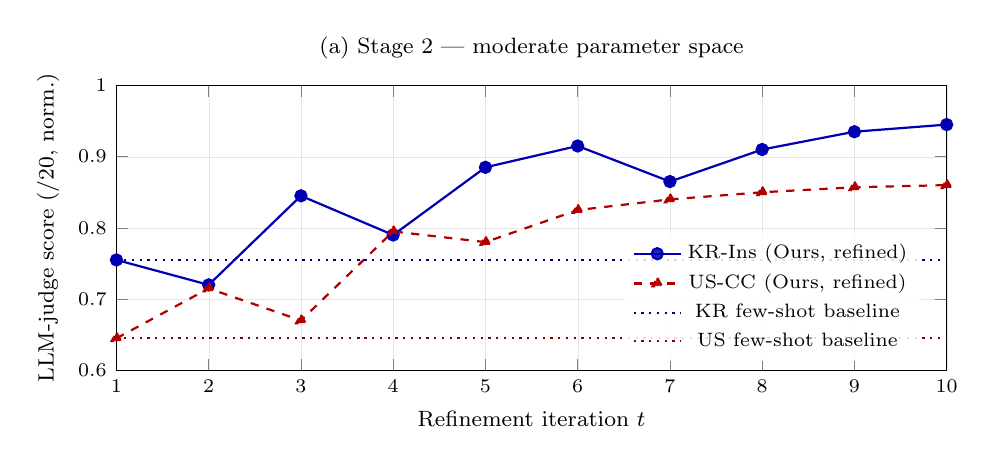
\begin{tikzpicture}
  \begin{axis}[
    width=\linewidth, height=5.2cm,
    xlabel={Refinement iteration $t$},
    ylabel={LLM-judge score (/20, norm.)},
    xmin=1, xmax=10, ymin=0.60, ymax=1.00,
    xtick={1,2,3,4,5,6,7,8,9,10},
    ytick={0.6,0.7,0.8,0.9,1.0},
    legend pos=south east,
    legend style={font=\scriptsize, draw=none, fill=white, fill opacity=0.85, text opacity=1},
    grid=both,
    grid style={line width=.1pt, draw=gray!20},
    tick label style={font=\scriptsize},
    label style={font=\footnotesize},
    title style={font=\footnotesize},
    title={(a) Stage 2 --- moderate parameter space},
  ]
  \addplot[mark=*,thick,color=blue!70!black] coordinates {
    (1,0.755) (2,0.720) (3,0.845) (4,0.790) (5,0.885)
    (6,0.915) (7,0.865) (8,0.910) (9,0.935) (10,0.945)
  };
  \addlegendentry{KR-Ins (Ours, refined)}
  \addplot[mark=triangle*,thick,color=red!70!black,dashed] coordinates {
    (1,0.645) (2,0.715) (3,0.670) (4,0.795) (5,0.780)
    (6,0.825) (7,0.840) (8,0.850) (9,0.857) (10,0.860)
  };
  \addlegendentry{US-CC (Ours, refined)}
  \addplot[domain=1:10,dotted,color=blue!50!black,thick] {0.755};
  \addlegendentry{KR few-shot baseline}
  \addplot[domain=1:10,dotted,color=red!50!black,thick] {0.645};
  \addlegendentry{US few-shot baseline}
  \end{axis}
  \end{tikzpicture}
\end{subfigure}
\hfill
\begin{subfigure}{0.48\textwidth}
  \centering
  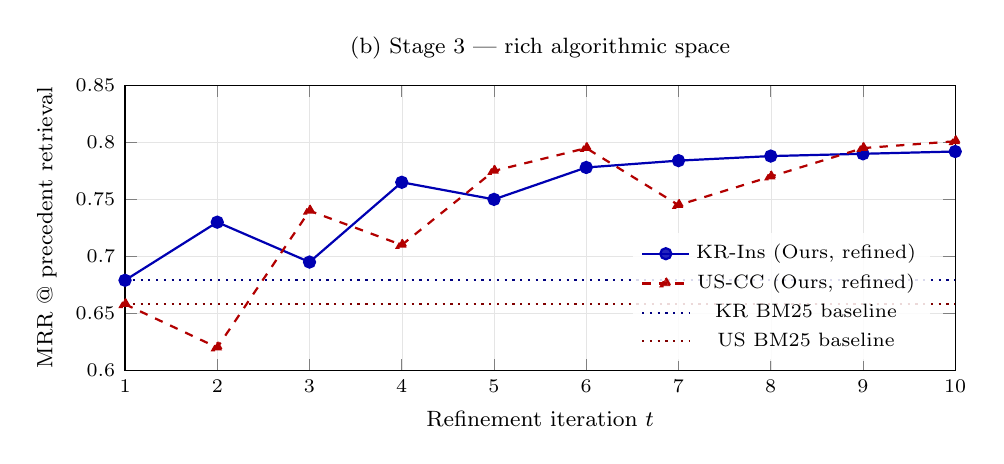
\begin{tikzpicture}
  \begin{axis}[
    width=\linewidth, height=5.2cm,
    xlabel={Refinement iteration $t$},
    ylabel={MRR @ precedent retrieval},
    xmin=1, xmax=10, ymin=0.60, ymax=0.85,
    xtick={1,2,3,4,5,6,7,8,9,10},
    ytick={0.6,0.65,0.7,0.75,0.8,0.85},
    legend pos=south east,
    legend style={font=\scriptsize, draw=none, fill=white, fill opacity=0.85, text opacity=1},
    grid=both,
    grid style={line width=.1pt, draw=gray!20},
    tick label style={font=\scriptsize},
    label style={font=\footnotesize},
    title style={font=\footnotesize},
    title={(b) Stage 3 --- rich algorithmic space},
  ]
  \addplot[mark=*,thick,color=blue!70!black] coordinates {
    (1,0.679) (2,0.730) (3,0.695) (4,0.765) (5,0.750)
    (6,0.778) (7,0.784) (8,0.788) (9,0.790) (10,0.792)
  };
  \addlegendentry{KR-Ins (Ours, refined)}
  \addplot[mark=triangle*,thick,color=red!70!black,dashed] coordinates {
    (1,0.658) (2,0.620) (3,0.740) (4,0.710) (5,0.775)
    (6,0.795) (7,0.745) (8,0.770) (9,0.795) (10,0.801)
  };
  \addlegendentry{US-CC (Ours, refined)}
  \addplot[domain=1:10,dotted,color=blue!50!black,thick] {0.679};
  \addlegendentry{KR BM25 baseline}
  \addplot[domain=1:10,dotted,color=red!50!black,thick] {0.658};
  \addlegendentry{US BM25 baseline}
  \end{axis}
  \end{tikzpicture}
\end{subfigure}
\caption{\textbf{Inherited Stage~2/3 iteration trace; not reproduced.} The original plot is retained for reconciliation, not as evidence on the fixed 3,000-source cohort. Its KR endpoints (18.9/20 and MRR 0.792) conflict with the inherited E2/E3 table values (17.3/20 and 0.575). No ten-iteration convergence or agreement with Tables~\ref{tab:e2}--\ref{tab:e3} is established by the current run.}
\label{fig:iter-trace}
\end{figure*}

\begin{table*}[t]
\centering
\small
\setlength{\tabcolsep}{4pt}


\begin{tabular}{llccccc}
\toprule
Dom. & Method & Trig. & Desc. & Query & Cov. & Total \\
\midrule
\multirow{5}{*}{KR-Ins}
  & Zero-shot (multimodal)  & 1.1 & 1.0 & 1.0 & 1.2 &  4.3/20 \\
  & OCR -- text (raw)       & 3.8 & 3.7 & 3.4 & 3.9 & 14.8/20 \\
  & Few-shot (FS)           & 3.9 & 3.6 & 3.8 & 3.8 & 15.1/20 \\
  & Ours (w/o refine)       & 3.9 & 3.8 & 3.7 & 4.0 & 15.4/20 \\
  & \textbf{Ours}           & 4.4 & 4.3 & 4.2 & 4.4 & \textbf{17.3/20} \\

\midrule
\multirow{5}{*}{US-CC}
  & Zero-shot (multimodal)  & 1.0 & 1.0 & 1.0 & 1.1 &  4.1/20 \\
  & OCR -- text (raw)       & 2.9 & 2.9 & 2.8 & 3.2 & 11.8/20 \\
  & Few-shot (FS)           & 3.1 & 3.3 & 3.0 & 3.5 & 12.9/20 \\
  & Ours (w/o refine)       & 3.2 & 3.1 & 3.2 & 3.6 & 13.1/20 \\
    & \textbf{Ours}           & 4.2 & 4.3 & 4.1 & 4.6 & \textbf{17.2/20} \\
\midrule
\multirow{4}{*}{US-Ln}
  & OCR -- text (raw)       & 2.7 & 3.1 & 1.0 & 1.7 &  8.6/20 \\
  & Few-shot (FS)           & 1.4 & 2.4 & 1.0 & 1.3 &  6.1/20 \\
  & Ours (w/o refine)       & 2.3 & 2.4 & 1.0 & 1.9 &  7.6/20 \\
  & \textbf{Ours}           & 2.1 & 3.3 & 3.3 & 1.7 & \textbf{10.4/20} \\
\bottomrule
\end{tabular}
\caption{\textbf{E2 --- Inherited input-format comparison; not reproduced.}
These are earlier manuscript values, not measurements on the fixed 3,000 sources.
The earlier draft attributes these four-axis scores to Claude Sonnet 4.5 and
GPT-4o judges; that execution and averaging protocol are not verified here.
}
\label{tab:e2}
\end{table*}

\begin{table*}[t]
\centering
\small
\setlength{\tabcolsep}{2pt}


\begin{tabular}{llccccc}
\toprule
Dom. & Method & MRR & P@1  & P@3 & R@3 & R@5 \\
\midrule
\multirow{5}{*}{KR-Ins}
  & BM25          & 0.492          & 0.286          & 0.254          & 0.714          & 0.810 \\
  & TF-IDF        & 0.431          & 0.190          & 0.222          & 0.667          & 0.762 \\
  & Emb.          & 0.447          & 0.238          & 0.238          & 0.690          & 0.786 \\
  & Hybrid        & 0.511          & 0.333          & 0.270          & 0.738          & 0.833 \\
  & \textbf{Ours} & \textbf{0.575} & \textbf{0.381} & \textbf{0.349} & \textbf{0.810} & \textbf{0.905} \\
\midrule
\multirow{5}{*}{US-CC}
  & BM25          & 0.658          & 0.287          & 0.271          & 0.416          & 0.455 \\
  & TF-IDF        & 0.724          & 0.259          & 0.311          & 0.361          & 0.446 \\
  & Emb.          & 0.741          & 0.271          & 0.324          & 0.378          & 0.463 \\
  & Hybrid        & 0.769          & 0.346          & 0.314          & 0.434          & 0.511 \\
  & \textbf{Ours} & \textbf{0.801} & 0.294          & \textbf{0.359} & \textbf{0.474} & \textbf{0.587} \\
\midrule
\multirow{5}{*}{US-Ln}
  & BM25          & 0.750          & 0.643          & 0.738          & 0.857          & 0.881 \\
  & TF-IDF        & 0.839          & 0.786          & 0.810          & 0.857          & 0.929 \\
  & Emb.          & 0.831          & 0.762          & 0.795          & 0.833          & 0.905 \\
  & Hybrid        & 0.836          & 0.786          & 0.786          & 0.857          & 0.929 \\
  & \textbf{Ours} & \textbf{0.964} & \textbf{0.929} & \textbf{0.905} & \textbf{1.000} & \textbf{1.000} \\
\bottomrule
\end{tabular}
\caption{\textbf{E3 --- Inherited retrieval comparison; not reproduced.}
These values do not describe the new 3,000-source experiment.
KR-Ins: 17-precedent pool from \texttt{data/precedents.json};
US-CC: CourtListener API; US-Ln: in-domain retrieval pool of 663
covenant-tagged paragraph chunks from 216 SEC loan agreements. All $\uparrow$.
The earlier draft labels the final row as a selected configuration; that
selection and its relevance labels are not verified here.}
\label{tab:e3}
\end{table*}

\begin{table*}[t]
\centering\small\setlength{\tabcolsep}{3.25pt}


\begin{tabular}{lcccccc}
\toprule
 & \multicolumn{2}{c}{KR-Ins} & \multicolumn{2}{c}{US-CC} & \multicolumn{2}{c}{US-Ln} \\
\cmidrule(lr){2-3}\cmidrule(lr){4-5}\cmidrule(lr){6-7}
Method & MRR & $\Delta$ & MRR & $\Delta$ & MRR & $\Delta$ \\
\midrule
Single-agent         & 0.531 & ---          & 0.763 & ---          & 0.871 & --- \\
w/o Meta-review      & 0.548 & +1.7         & 0.779 & +1.6         & 0.903 & +3.2 \\
w/o Evolution        & 0.554 & +2.3         & 0.784 & +2.1         & 0.918 & +4.7 \\
\textbf{Full (Ours)} & \textbf{0.575} & \textbf{+4.4} & \textbf{0.801} & \textbf{+3.8} & \textbf{0.964} & \textbf{+9.3} \\
\bottomrule
\end{tabular}
\caption{\textbf{E4 --- Inherited Stage~3 ablation; not reproduced.}
The following interpretation is an unverified earlier claim:
Removing either supporting agent degrades final MRR across all
three tasks; the full three-agent loop achieves the largest gains.
$\Delta$ denotes absolute MRR change relative to the
single-agent baseline.}
\label{tab:e4}
\end{table*}

\begin{table*}[t]
\centering\small\setlength{\tabcolsep}{5pt}


\begin{tabular}{lcc}
\toprule
Method & Proposed & Precision $\uparrow$ \\
\midrule
Few-shot (FS)         & 4.2 & 0.531 \\
Ours (w/o refine)     & 5.1 & 0.614 \\
\textbf{Ours}         & 4.7 & \textbf{0.823} \\
\bottomrule
\end{tabular}
\caption{\textbf{E5 --- Inherited human assessment; trace not established.}
Not verified precision or a current 3,000-source result.
The earlier draft claims 120 sampled contracts and defines precision as
validated candidates / total proposed; the annotation trace is not established.}
\label{tab:e5}
\end{table*}

\begin{figure*}[t]
    \centering
    
\includegraphics[width=0.9\textwidth]{FILE.png}
    \caption{\textbf{Preserved historical directory diagram.}
This image is a design artifact, not the executed file layout.
The actual TXT harness and current Stage~1 entry point are described in
Appendix~\ref{sec:implementation}. No Stage~2/3 evolution trace is established.}
    \label{fig:file}
\end{figure*}

\end{document}
